\chapter{Temporal}
    \section{Setup del proyecto}
    \subsection{CI/CD}
        
        CI/CD es un concepto de Ingeniería de Software, relacionado estrechamente con la filosofía \textit{DevOps} y con las metodologías ágiles; en el que se implementan flujos de trabajo que permitan distribuir las aplicaciones a los clientes de forma rápida, continua y fiable, a través de la automatización de ciertas etapas del desarrollo software.
        
        El nombre es una combinación de dos siglas, las cuales tienen diferentes significados: CI hace referencia a \textit{Continuous Integration} (integración continua), mientras que CD puede indicar dos procesos distintos: bien \textit{Continuous Delivery} (entrega continua) o \textit{Continuous Deployment} (despliegue continuo), los cuales en ocasiones se utilizan indistintamente.
        
        Ahondando en dichos conceptos, la integración continua es un proceso por el cual se
        establece un único repositorio central, el cual contiene tanto el código del producto software como sus pruebas unitarias y de integración. Tras ello se establece una capa de automatización que permite realizar la integración, construcción y pruebas del software en cada actualización del repositorio. 
        
        Por otra parte, la entrega y despliegue continuo tienen en común la automatización de las etapas de puesta en marcha del nuevo software. No obstante, la entrega continua aboga por un despliegue manual de los artefactos al no necesitarse o no ser beneficioso cambios frecuentes en el entorno de producción, mientras que el despliegue continuo automatiza dicho despliegue. Por tanto, el uso de un proceso u otro reside en las necesidades del proyecto.
        
        La implementación de una infraestructura CI/CD permite a los desarrolladores entregar cambios de forma rápida al reducir enormemente el tiempo de integración y despliegue, incrementando la eficiencia y eficacia en la implementación de software. 
        
        Asimismo, permite a los miembros del equipo trabajar de forma simultánea en distintas partes del software, sin tener que parar para la integración de todos los cambios y resolver los conflictos que puedan aparecer.
    
    \section{Sprint \#0}
        Este sprint se desarrolló entre el 5 y el 21 de septiembre, y consistió en la selección y puesta en marcha de las herramientas que se utilizarían para el desarrollo de este proyecto.
        
        \subsection{Notion}
            Notion es una plataforma online parcialmente gratuita utilizada para el seguimiento de proyectos y de equipos, la cual es fácilmente personalizable a partir de una serie de elementos predefinidos, entre los que se encuentran bases de datos embebidas (y vistas visuales como las mismas, como tableros Kanban o diagramas Gantt), soporte para imágenes, vídeo y audio, integración con otras plataformas como Slack, Zoom, Twitter...
            
            En esta herramienta se pueden construir páginas, las cuales pueden contener texto formateado con el lenguaje de marcado Markdown o cualquiera de los bloques anteriores, por lo que fue elegida para conformar el centro neurálgico del seguimiento del proyecto.
            
            Se implementaron los siguientes elementos
            
            \begin{itemize}
                \item Tablero Kanban. Aquí son almacenadas las tareas del proyecto, con atributos sobre su estado, su categoría y sus fechas de desarrollo.
                    \begin{figure}[h!]
                        \centering
                        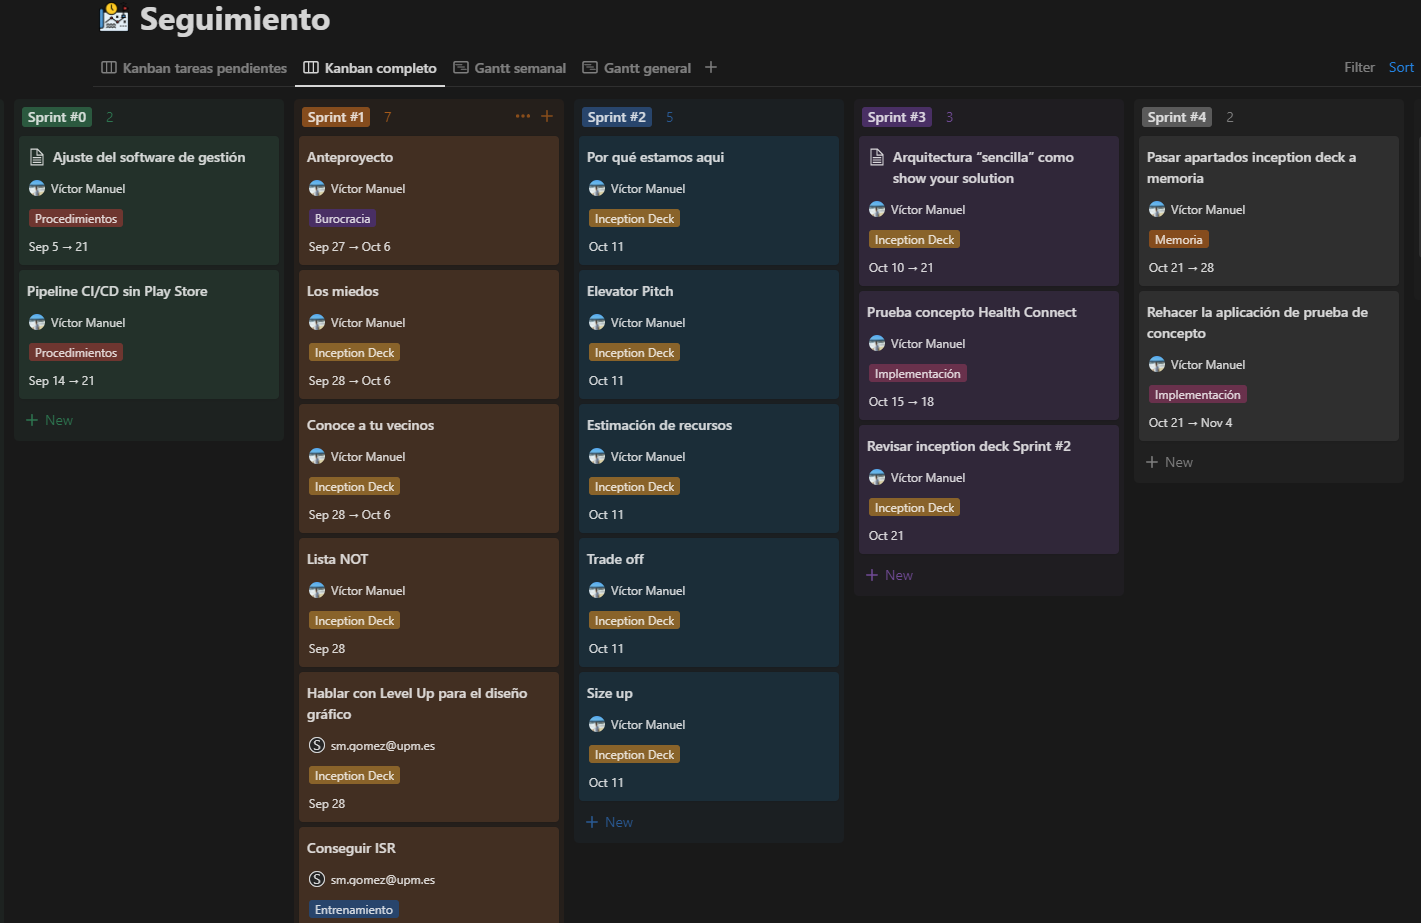
\includegraphics[width=0.75\textwidth]{figures/s0/Kanban completo.PNG}
                        \caption{Extracto del tablero Kanban del proyecto}
                        \label{fig:notion:kanban}
                    \end{figure}
                \item Diagrama Gantt. En esencia es una vista a la misma base de datos que la del tablero Kanban.
                    \begin{figure}[h!]
                        \centering
                        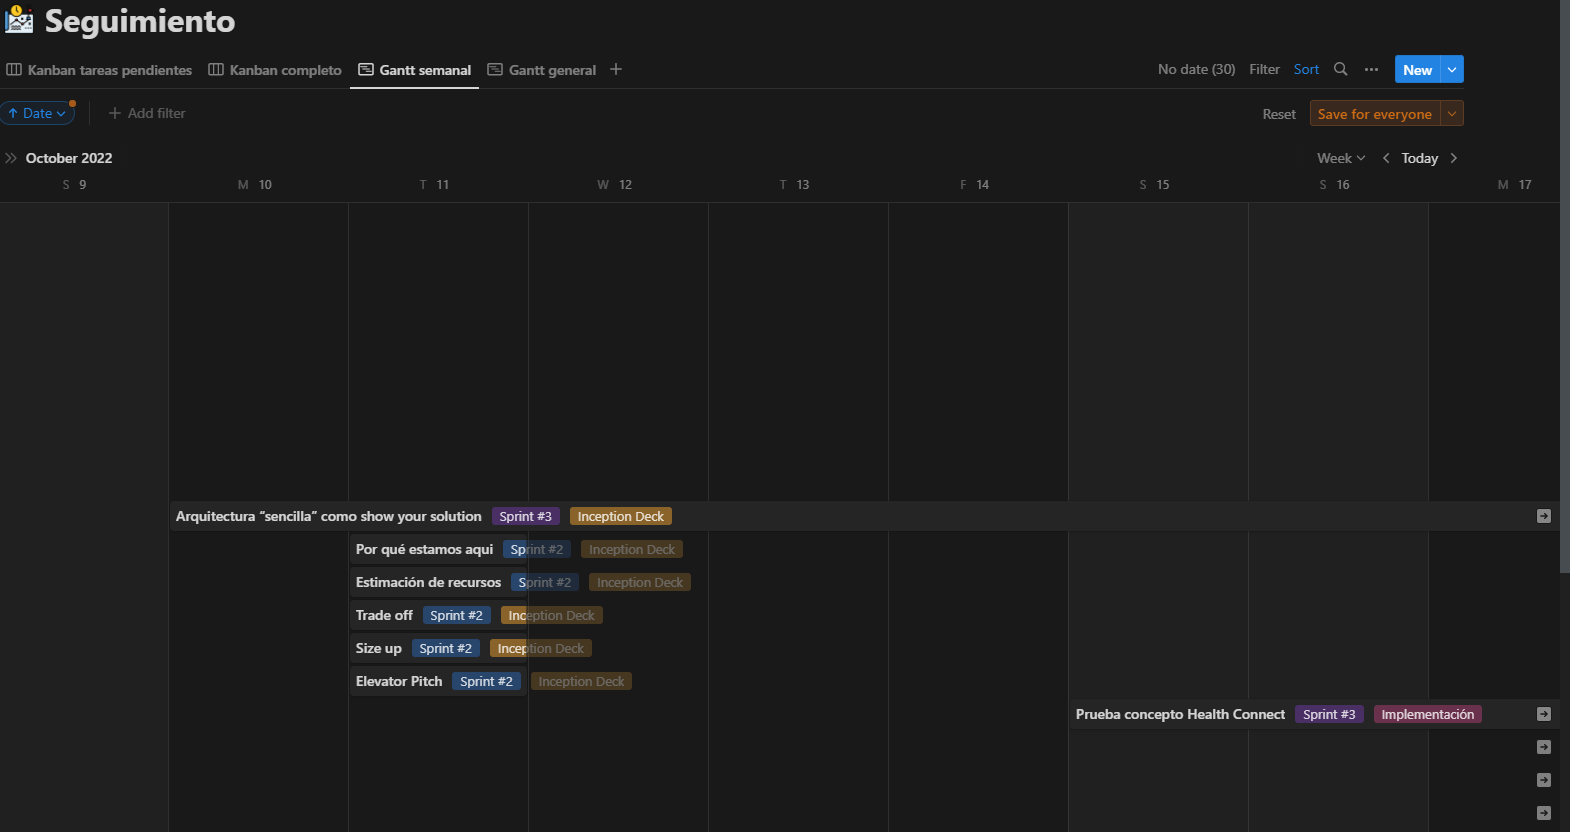
\includegraphics[width=0.75\textwidth]{figures/s0/gantt semanal.PNG}
                        \caption{Extracto del diagrama Gantt del proyecto}
                        \label{fig:notion:gantt}
                    \end{figure}
                \item Base de datos de referencias con todos los link de interés para la implementación del proyecto. Algunos de ellos aparecen en la bibliografía de esta memoria por su relevancia para exponer ciertas cuestiones.
                    \begin{figure}[h!]
                        \centering
                        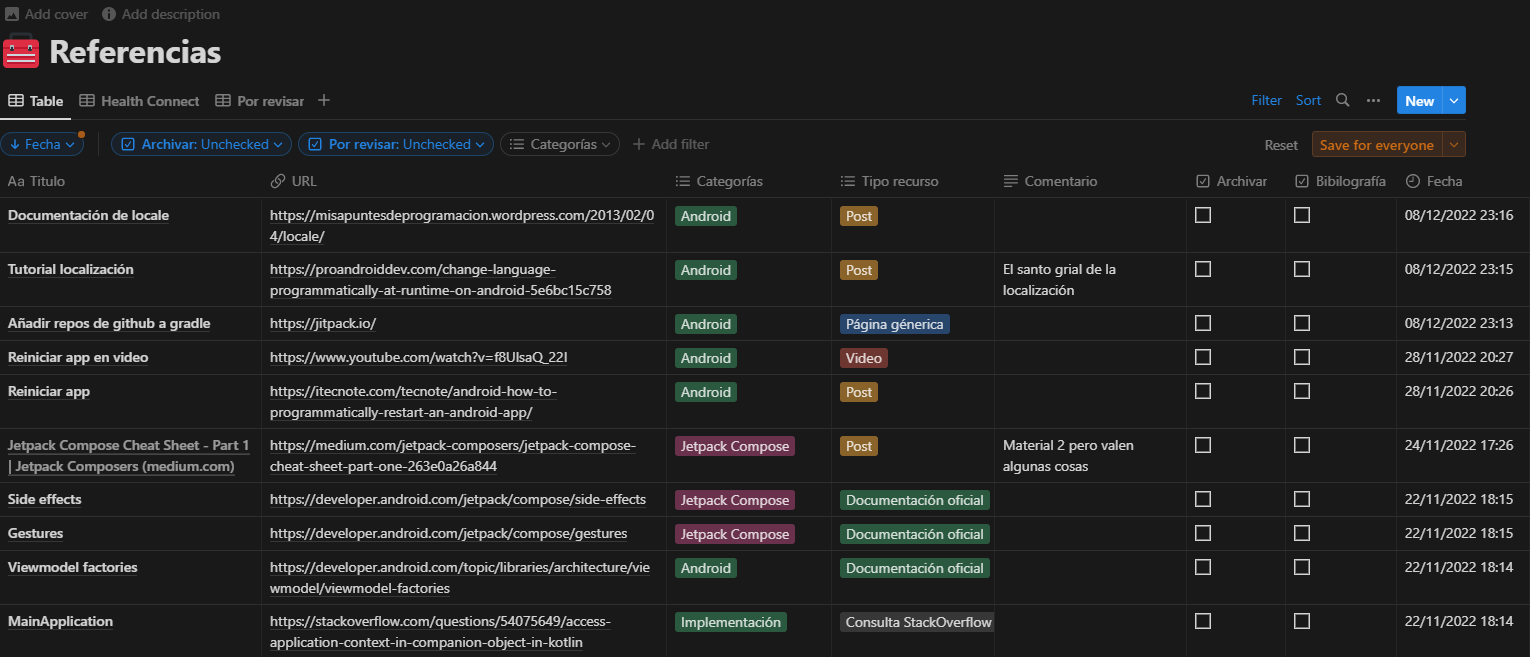
\includegraphics[width=0.75\textwidth]{figures/s0/referencias.PNG}
                        \caption{Extracto de la base de datos de referencias}
                        \label{fig:notion:referencias}
                    \end{figure}
                \item Base de datos con apuntes de consulta. Aquí se alojan descripciones de conceptos de utilidad para el proyecto. Está enlazada con la base de datos de referencia para acceder rápidamente a los enlaces para ampliar esa información.
                    \begin{figure}[h!]
                        \centering
                        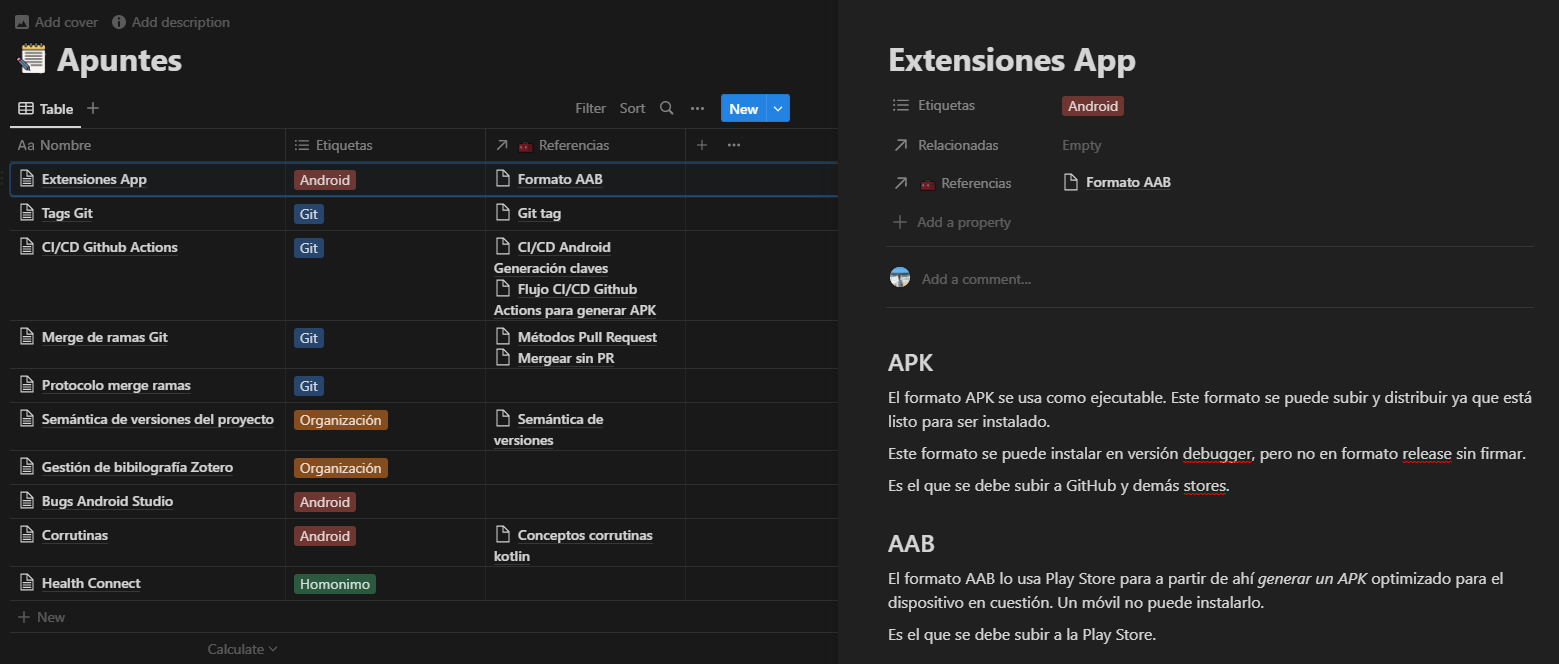
\includegraphics[width=0.75\textwidth]{figures/s0/apuntes.PNG}
                        \caption{Extracto de la base de datos de apuntes del proyecto}
                        \label{fig:notion:apuntes}
                    \end{figure}
            \end{itemize}
            
        \subsection{Microsoft Teams}
            Microsoft Teams es una herramienta de comunicación y colaboración para equipos propiedad de Microsoft. Es principalmente utilizada para alojar canales de comunicación y videollamadas.
            
            Para este proyecto lo hemos seleccionado por dos de sus funcionalidades: desplegar un sistema de archivos en la nube para cada canal de comunicación y registro de turnos de trabajo.
            
            En cuanto a la primera de ellas, la hemos elegido por delante de otras opciones de alojamiento ya que por ser usuarios de la UPM, disponemos de 1 TB de almacenamiento, por lo que podemos alojar todo tipo de contenido multimedia prácticamente sin restricciones y de forma fácil y sencilla.
            
            \begin{figure}[h!]
                \centering
                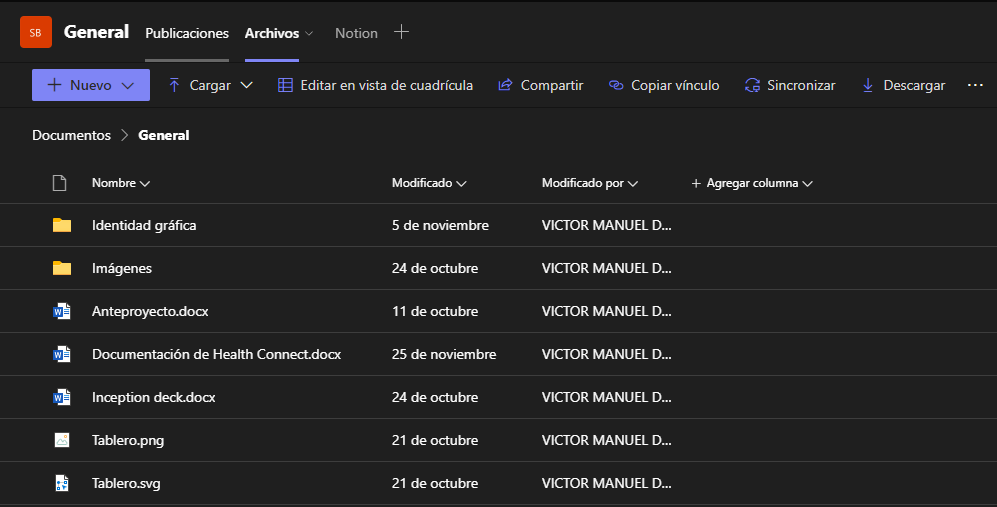
\includegraphics[width=0.75\textwidth]{figures/s0/archivos teams.PNG}
                \caption{Extracto de los documentos alojados en Teams}
                \label{fig:teams:documentos}
            \end{figure}
            
            Asimismo, la funcionalidad de registro de turnos es cómoda de usar y nos genera automáticamente un excel con las horas registradas por parte de todos los miembros del equipo, ideal si queremos registrar el total de horas empleadas en el proyecto.
            
        
        \subsection{Zotero}
            Zotero es una plataforma open-source (licenciado con AGPL) de gestión de referencias y citas bibliográficas, que permite recopilar y almacenar referencias de libros, artículos, sitios web y otros documentos cómodamente. Una vez registradas, permite exportar dichas citas de acuerdo a diferentes estilos de citación.
            
            En este proyecto ha sido seleccionada por su facilidad de uso, por ser open-source y disponer de una gran cantidad de plugins, como \textit{Zotero Connector}, que nos permite agregar referencias desde el navegador.
            
        
        \subsection{Git y Github}
        
            Git es sistema de control de versiones open-source (bajo la licencia GNU GPL v2) diseñado por Linus Torvalds, siendo muy popular entre los equipos de desarrollo software. Si bien Git almacena y gestiona cambios en archivos de cualquier tipo, está pensado para ser más eficiente en los archivos de código fuente.
            
            Por otra parte, Github es una plataforma en línea que ofrece alojamiento y gestión de proyectos que utilicen Git. Para este proyecto, además del alojamiento, utilizamos sus herramientas de CI/CD (GitHub Actions), por la que a través de un fichero .yml podemos configurar un pipeline de acciones con las que realizar los procesos que queramos automáticamente. Además, pueden establecerse flujos de trabajos por ramas de desarrollo u otras condiciones, tales como formatos de tags, tipos de eventos...
            
        
        \subsection{\LaTeX y Overleaf}
        \LaTeX como medio de creación de la presente memoria y Overleaf como editor de dicho lenguaje.


    \section{Tecnologías}
        \subsection{Jetpack Compose}
            Jetpack Compose es el conjunto de herramientas \textit{modernas} de Android para el desarrollo de interfaces gráficas, lanzado en su primera versión estable el 28 de julio de 2021 por Google. Este kit de librerías permite desarrollar en el ecosistema Android de forma nativa interfaces gráficas de manera declarativa como en los sistemas React, Flutter o SwiftUI, siguiendo las tendencias actuales de la industria en el desarrollo de aplicaciones móviles.

            Hasta la aparición de Jetpack Compose, el desarrollo interfaces gráficas nativas en Android se realizaba con el enfoque conocido como programación imperativa. En este tipo de desarrollo es necesario especificar paso por paso cómo se va a construir dicha interfaz gráfica. En dicho proceso (conocido en Android como sistema de vistas) se codificaba un fichero XML, en el que se describían todos los elementos gráficos (botones, textos...); para en el código Java (o Kotlin) de la aplicación se accediera a dichos elementos y se le aplicaran modificaciones y transformaciones de manera totalmente manual.

            En Jetpack Compose la interfaz está interconectada a un estado, por lo que si dicho estado cambia, nuestra interfaz gráfica cambiará para mostrar el nuevo estado, simplificando enormemente el desarrollo y reduciendo el código necesario. Asimismo, a diferencia del sistema anterior, está desacoplada del sistema operativo, por lo que no dependemos de la versión del terminal para ejecutar correctamente nuestra interfaz gráfica, como si ocurría anteriormente. Por último, Jetpack Compose es compatible con los componentes XML del sistema anterior, lo que facilita la migración de los proyectos antiguos a este nuevo paradigma.

            No obstante, este conjunto de herramienta solo es compatible con el lenguaje de programación Kotlin, por lo que en algunos casos puede incrementarse la curva de dificultad para aprender a utilizarlo.

            ----------

            Para crear nuestras interfaces en Jetpack Compose crearemos funciones con la anotación Composable, la cual nos permite crear elementos gráficos dentro de su contenido, tales como botones, textos, imágenes..

            Para poder ver cómo va quedando nuestra interfaz gráfica tenemos que recurrir a las vistas previas. Estas funciones llevan la anotación Composable y una nueva conocida como Preview, la cual permite que se pueda visualizar su contenido de manera independiente a cambio de imponer una serie de restricciones. En esas funciones Preview llamamos a la función Composable que queremos visualizar.


    \section{Desarrollo}
        \subsection{Inyección de dependencias (Dagger Hilt)}
        \subsection{Cifrado de la base de datos (SQLCipher)}
        \subsection{Navegación entre ventanas (Compose Destination)}
        \subsection{Planificación de tareas (Work Manager)}
        \subsection{Comunicación con el servidor (Retrofit)}
        \subsection{Ajustes del usuario (Datastore)}
        \subsection{Localización de la app (Strings.xml y Lingliver)}
        \subsection{Onboarding (Lottie)}
        \subsection{Gráficas (Vico)}
        \subsection{Flujos de integración continua (GitHub Actions)}
            
            
            